% previous work and challenges
\section*{}
\subsection*{Motivation}

\begin{frame} %-----------------------------%
\frametitle{Previous Work} % small satellites
\framesubtitle{Challenges}
\begin{itemize}
	\item Optimal Trajectory Design
		\begin{itemize}
			\item Orbital dynamics are nonlinear and chaotic
			\item Very sensitive to initial conditions
			\item Intuition required by designer
		\end{itemize}
	\pause
	\item Direct Optimal Control
		\begin{itemize}
			\item Reformulate problem as parameter optimization
			\item Allows for use of nonlinear programming methods
			\item High dimensional problem and computationally intensive
		\end{itemize}
	\pause
	\item Numerical Integration
		\begin{itemize}
			\item Typical methods use Runge-Kutta schemes
			\item Numerical Instability and Energy drift
			\item Difficult to capture  long-term effects of low-thrust propulsion accurately
		\end{itemize}
	\pause
	\item Invariant Manifolds
		\begin{itemize}
			\item Associated with periodic orbits
			\item Control-free and transfers require manifolds to intersect
		\end{itemize}
\end{itemize}
\end{frame}   %-----------------------------%

%\begin{frame} %-----------------------------%
%\frametitle{Previous Work}
%\framesubtitle{Challenges}
%\begin{itemize}
%	\item Invariant manifolds of three-body problem used for transfers
%	\item Generated from periodic orbits in three-body problem
%	\item Results are case specific and difficult to generalize
%	\item Control-free and dependent on intersections of manifolds
%	\item Long time of flight not conducive for time critical missions
%	
%	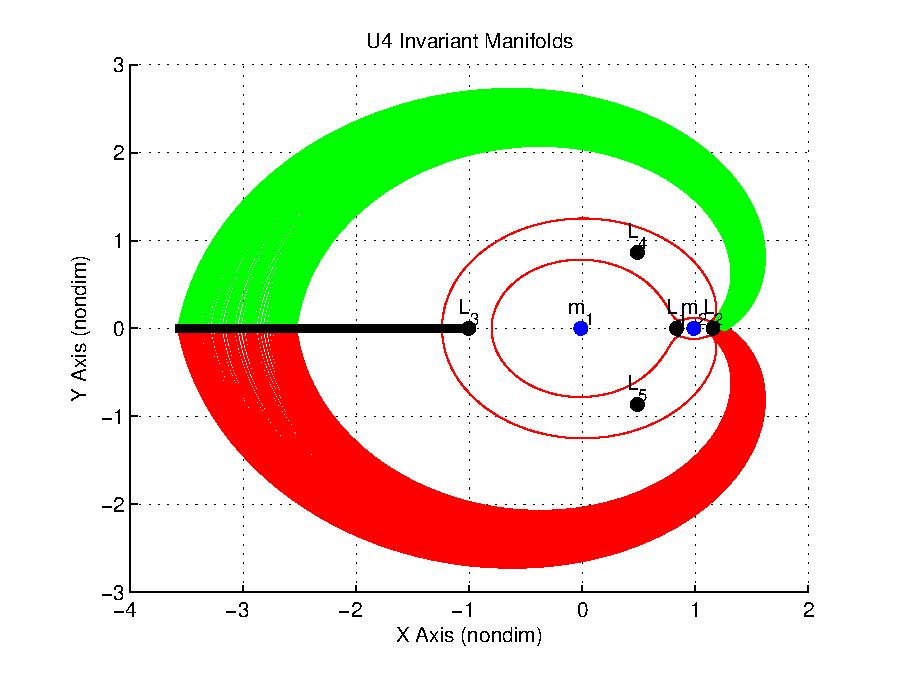
\includegraphics[height=0.3\textheight]{U4_Manifolds}
%	\hfill
%	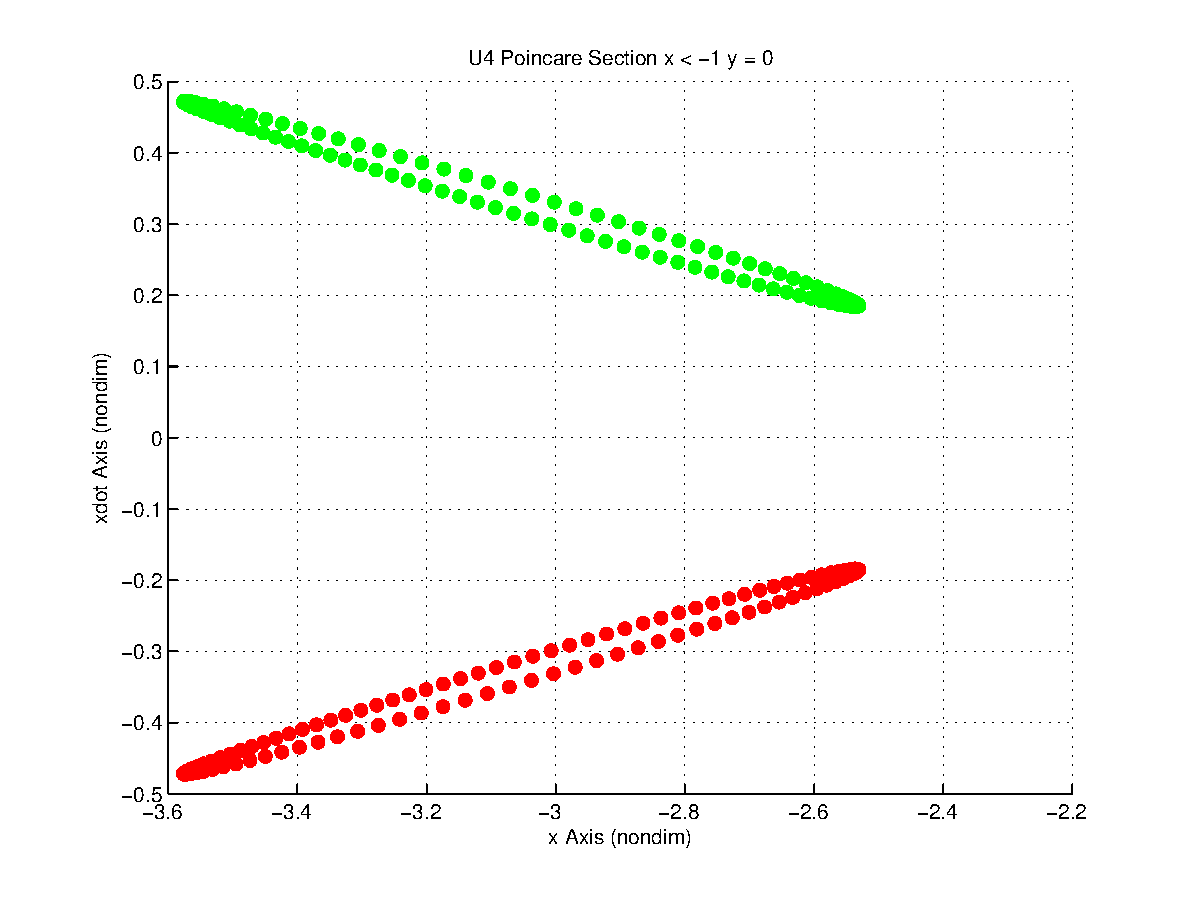
\includegraphics[height=0.3\textheight]{U4_poincare}
%\end{itemize}
%\end{frame} %--------------------------------%

\begin{frame} % -----------------------------------%
\frametitle{Proposed Approach}
		\begin{itemize}
			\item Extend invariant manifold concept with low-thrust control  
			\item Variational integrator allows for accurate and stable computation
			\item \emph{Computational geometric optimal control} used to generate reachable set
			\item \emph{Reachability set} on Poincar\'e section allows for systematic transfer design
		\end{itemize}
\end{frame} %--------------------------------------%